\documentclass[portrait,final,a0paper]{baposter}
%\documentclass[a4shrink,portrait,final]{baposter}
% Usa a4shrink for an a4 sized paper.

\tracingstats=2
\usepackage{calc}
\usepackage{graphicx}
\usepackage{amsmath}
\usepackage{amssymb}
\usepackage{relsize}
\usepackage{multirow}
\usepackage{bm}

\usepackage{graphicx}


\usepackage{pgfbaselayers}
\pgfdeclarelayer{background}
\pgfdeclarelayer{foreground}
\pgfsetlayers{background,main,foreground}

\usepackage{times}
\usepackage{helvet}
%\usepackage{bookman}
\usepackage{palatino}
\usepackage{background}

\newcommand{\captionfont}{\footnotesize}

\selectcolormodel{cmyk}

\graphicspath{{images/}}


%%%%%%%%%%%%%%%%%%%%%%%%%%%%%%%%%%%%%%%%%%%%%%%%%%%%%%%%%%%%%%%%%%%%%%%%%%%%%%
%%% Begin of Document
%%%%%%%%%%%%%%%%%%%%%%%%%%%%%%%%%%%%%%%%%%%%%%%%%%%%%%%%%%%%%%%%%%%%%%%%%%%%%%


\begin{document}
\typeout{Poster rendering started}	

\SetBgContents{}
%%% Setting Background Image %%%%%%%%%%%%%%%%%%%%%%%%%%%%%%%%%%%%%%%%%%%%%%%%%%
\background{
	\begin{tikzpicture}[remember picture,overlay]%
	\draw (current page.center)+(-1em,1em) node[anchor=center,opacity=0.2, scale=1.1]
	{\includegraphics[width=1.1\textwidth]{background1}};
	\end{tikzpicture}
}	

%%%%%%%%%%%%%%%%%%%%%%%%%%%%%%%%%%%%%%%%%%%%%%%%%%%%%%%%%%%%%%%%%%%%%%%%%%%%%%
%%% Here starts the poster
%%%---------------------------------------------------------------------------
%%% Format it to your taste with the options
%%%%%%%%%%%%%%%%%%%%%%%%%%%%%%%%%%%%%%%%%%%%%%%%%%%%%%%%%%%%%%%%%%%%%%%%%%%%%%
% Define some colors
\definecolor{DarkMagenta}{cmyk}{0,0.64,0.2,0}
\definecolor{yellow}{cmyk}{0.3,0.1,0.2,0.0}
\definecolor{reddishyellow}{cmyk}{0,0.22,1.0,0.0}
\definecolor{black}{cmyk}{0,0,0.0,1.0}
\definecolor{darkYellow}{cmyk}{0,0,1.0,0.5}
\definecolor{Carnelian}{cmyk}{1.0,0.29,0.0,0.26}

\definecolor{lightyellow}{cmyk}{0.0,0.0,0.0,0.0}
\definecolor{lighteryellow}{cmyk}{0,0,0.0,0.0}
\definecolor{lighteryellow}{cmyk}{0,0,0.0,0.0}
\definecolor{lightestyellow}{cmyk}{0,0,0.0,0.0}

\definecolor{primary1}{cmyk}{0.5,1.0,0.0,0.0}
\definecolor{primary2}{cmyk}{0,0,0,0.5}
\definecolor{primary3}{cmyk}{0,0,0,0.8}

\definecolor{secondary1}{cmyk}{0.82,0.38,0.2,0.2}
\definecolor{secondary2}{cmyk}{0.91,0.91,0.6,0.18}
\definecolor{secondary3}{cmyk}{0.71,0.23,0.13,0.3}
\definecolor{secondary4}{cmyk}{0.38,0.16,0.0,0.0}
\definecolor{secondary5}{cmyk}{0.20,0.62,0.2,0.0}
\definecolor{secondary6}{cmyk}{0.63,0.2,0.26,0.0}

%%
%\typeout{Poster Starts}

\newlength{\leftimgwidth}
\begin{poster}%
  % Poster Options
  {
  % Show grid to help with alignment
  grid=false,
  % Column spacing
  colspacing=1em,
  % Color style
  bgColorOne=lightestyellow,
  bgColorTwo=lightestyellow,
  borderColor=primary2,
  headerColorOne=primary1,
  headerColorTwo=reddishyellow,
  headerFontColor=white,
  boxColorOne=lightyellow,
  boxColorTwo=lighteryellow,
  % Format of textbox
  textborder=roundedleft,
%  textborder=rectangle,
  % Format of text header
  eyecatcher=false,
  headerborder=open,
  headerheight=0.095\textheight,
  headershape=roundedright,
  headershade=plain,
  headerfont=\Large\sf\bf, %Sans Serif
 % boxshade=plain,
%  background=shade-tb,
  background=user,
  linewidth=1.6pt
  }
  % Eye Catcher
  {\includegraphics[width=10em]{background1.png}} % No eye catcher for this poster. (eyecatcher=no above). If an eye catcher is present, the title is centered between eye-catcher and logo.
  % Title
  {
  \vspace{2.2em}
  \color{primary1}
  \textbf{
  Classification of Cells Based on Scale-space Measures and Semi-supervised Machine Learning}
  }
  % Authors
  {
  % Serif
  \vspace{0.5em}\textbf{\ S. Vohra\textsuperscript{2}, L. Antanas\textsuperscript{2}, L. Raedt\textsuperscript{2} and D. Prodanov\textsuperscript{1}}\\
   \textsuperscript{1}EHS, Imec, Leuven, Belgium, \textsuperscript{2} KU Leuven\\
   \vspace{1.94em}
    
  }
  % University logo
  {% The makebox allows the title to flow into the logo, this is a hack because of the L shaped logo.  
  	 \makebox[11em][r]{%
  	 	\begin{minipage}{16em}
  	 		\hfill
  	 		
\includegraphics[height=7.8em]{imec_logo}
  	 	\end{minipage}
  	 }
  }
   
    
%%%%%%%%%%%%%%%%%%%%%%%%%%%%%%%%%%%%%%%%%%%%%%%%%%%%%%%%%%%%%%%%%%%%%%%%%%%%%%
%%% Now define the boxes that make up the poster
%%%---------------------------------------------------------------------------
%%% Each box has a name and can be placed absolutely or relatively.
%%% The only inconvenience is that you can only specify a relative position 
%%% towards an already declared box. So if you have a box attached to the 
%%% bottom, one to the top and a third one which should be in between, you 
%%% have to specify the top and bottom boxes before you specify the middle 
%%% box.
%%%%%%%%%%%%%%%%%%%%%%%%%%%%%%%%%%%%%%%%%%%%%%%%%%%%%%%%%%%%%%%%%%%%%%%%%%%%%%
    %
 
%%%%%%%%%%%%%%%%%%%%%%%%%%%%%%%%%%%%%%%%%%%%%%%%%%%%%%%%%%%%%%%%%%%%%%%%%%%%%%
  \headerbox{Context}{name=contribution,column=0,row=0, span=1}{
%%%%%%%%%%%%%%%%%%%%%%%%%%%%%%%%%%%%%%%%%%%%%%%%%%%%%%%%%%%%%%%%%%%%%%%%%%%%%%
\begin{itemize}
	\item Expert segment Anatomic \& Time Lapsed Images manually.
	\item Tools are very domain specific. 
	\item Most of the tools are based on original intensity which vary lot among images. 
\end{itemize}
	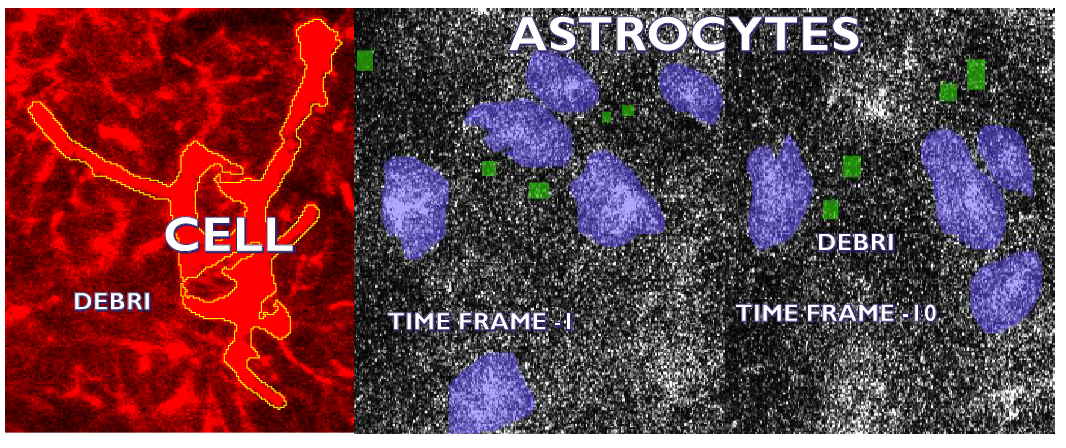
\includegraphics[width=.99\textwidth]{MONTAGE31}		

}


%%%%%%%%%%%%%%%%%%%%%%%%%%%%%%%%%%%%%%%%%%%%%%%%%%%%%%%%%%%%%%%%%%%%%%%%%%%%%%

\headerbox{Objective}{name=funding,column=1,span=2,row=0}{
	%%%%%%%%%%%%%%%%%%%%%%%%%%%%%%%%%%%%%%%%%%%%%%%%%%%%%%%%%%%%%%%%%%%%%%%%%%%%%%
	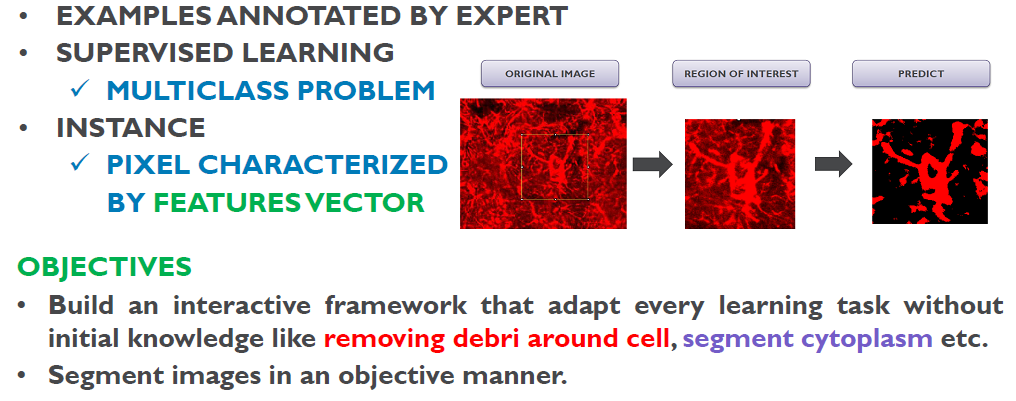
\includegraphics[width=.90\textwidth]{objective1}	
\begin{itemize}
	\item Build an interactive framework that adapt every learning task without initial knowledge like removing debris around cell,  segment cytoplasm etc.
	\item Segment images in an objective manner.
\end{itemize}
	
}

%%%%%%%%%%%%%%%%%%%%%%%%%%%%%%%%%%%%%%%%%%%%%%%%%%%%%%%%%%%%%%%%%%%%%%%%%%%%%%
  \headerbox{Features Extraction }{name=feature,column=0,below=contribution,span=3}{
%%%%%%%%%%%%%%%%%%%%%%%%%%%%%%%%%%%%%%%%%%%%%%%%%%%%%%%%%%%%%%%%%%%%%%%%%%%%%%

  	\includegraphics[width=.99\textwidth]{FEATURE2}


  }


%%%%%%%%%%%%%%%%%%%%%%%%%%%%%%%%%%%%%%%%%%%%%%%%%%%%%%%%%%%%%%%%%%%%%%%%%%%%%%
\headerbox{Method}{name=baseline,column=0,span=3,below=feature}{


			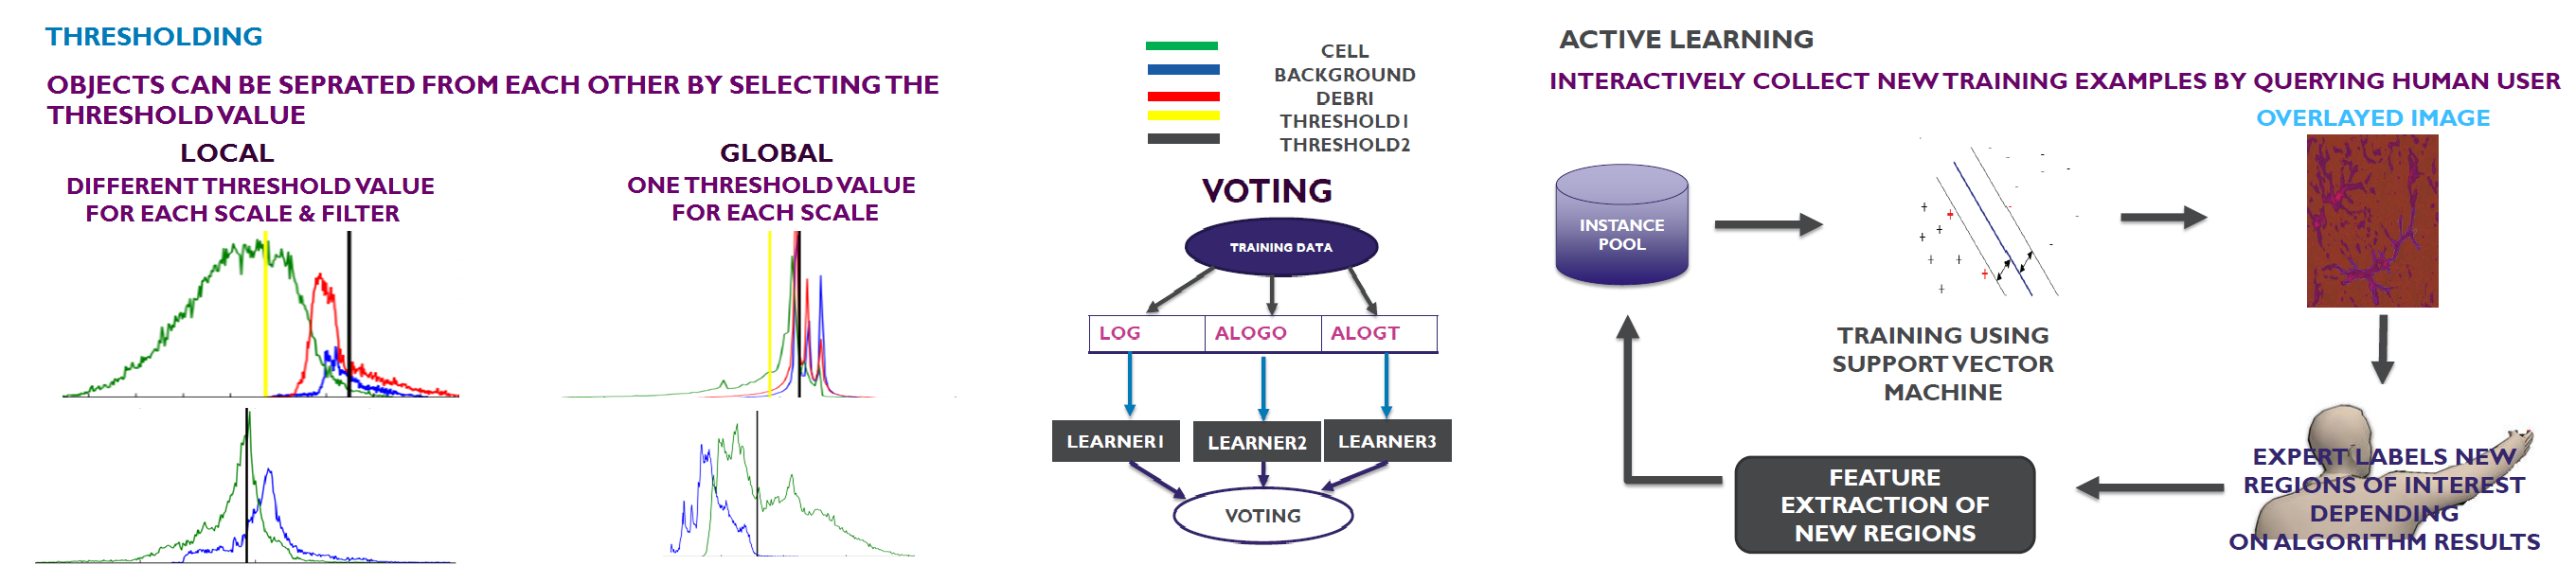
\includegraphics[width=.99\textwidth]{threshold12}
			
	
}

\headerbox{Evaluation}{name=evaluation,column=0,span=3,below=baseline}{
		
	
	\begin{minipage}{.55\textwidth}
		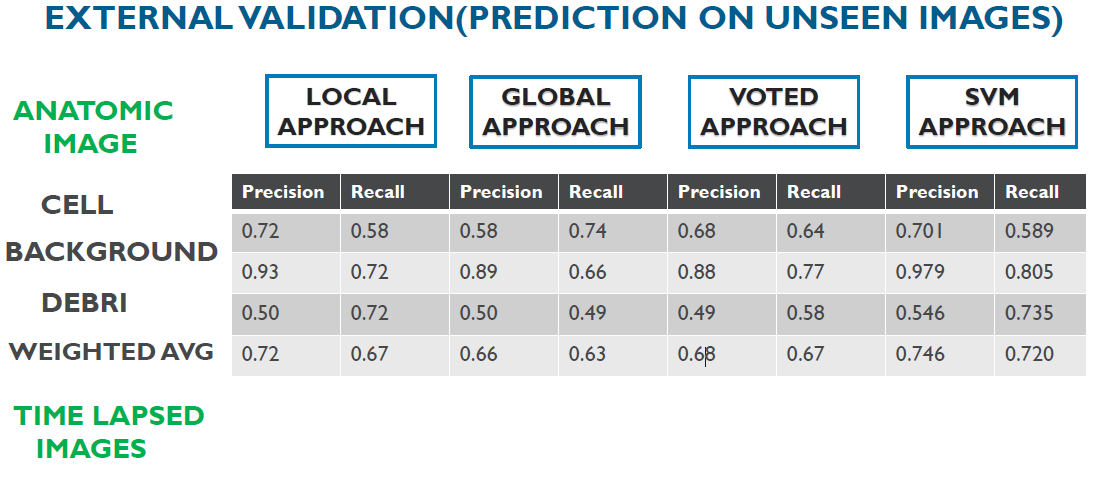
\includegraphics[width=.95\textwidth]{results12T}
		
	\end{minipage} 
		\begin{minipage}{.45\textwidth}
			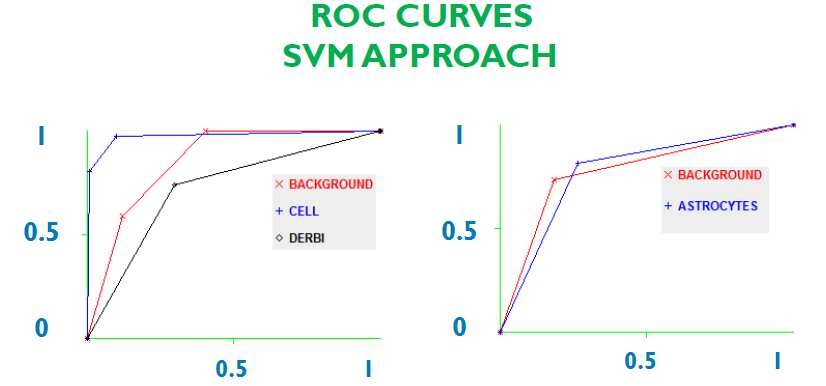
\includegraphics[width=.95\textwidth ]{results13}
		\end{minipage}
		
	
	
}
	\hspace{6 cm}
 \centerline{ 
 	\begin{minipage}{20em}
 		
\includegraphics[height=1.8em]{logo_kul}   		
 		\vspace{0.15cm}		
 	\end{minipage}
 		\begin{minipage}{20em}
 			
\includegraphics[height=2.4em]{imec_logo}   		
 			\vspace{0.15cm}		
 		\end{minipage}
 }

  
\end{poster}

\end{document}
